
\section{mcliqueInfo.rb Display Information on Clique Enumeration \label{sect:mcliqueInfo}}

This command displays information on clique enumerated from mclique.rb command. The main purpose is to generate information on connection relationship between cliques. 

Figure \ref{fig:mcinfo_1} shows the graph used for the illustration of mclique2g.rb command. 4 maximal cliques are obtained from this graph. For each of these four cliques, 5 types of information are generated as show in Table \ref{tbl:mcinfo_1}. 

\begin{table}[htbp]
\begin{center}
\caption{Output Results of this Command\label{tbl:mcinfo_1}}
%{\small
\begin{tabular}{lll}
\hline
Output Column name&Description& Example of id=1(\{$d,e,f$\}) \\
\hline
nSize      & Number of nodes                    & 3 (3 nodes $d,e,f$)\\
eSize      & Number of edges (nSize$*$(nSize-1)/2) & 3 $(3*2/2=3)$\\
extNodes   & Number of nodes with external connection            & 5 (Fig. \ref{fig:mcinfo_3} on right) \\
extEdges   & Number of edges with external connection              & 7 (Fig. \ref{fig:mcinfo_3} on left) \\
extCliques & Number of Cliques with external connection        & 3 (Fig. \ref{fig:mcinfo_2}) \\
\hline
\end{tabular} 
\end{center}
\end{table}


\begin{figure}[htbp]
\begin{center}
\begin{tabular}{cc}

\begin{minipage}{0.5\hsize}
\begin{center}
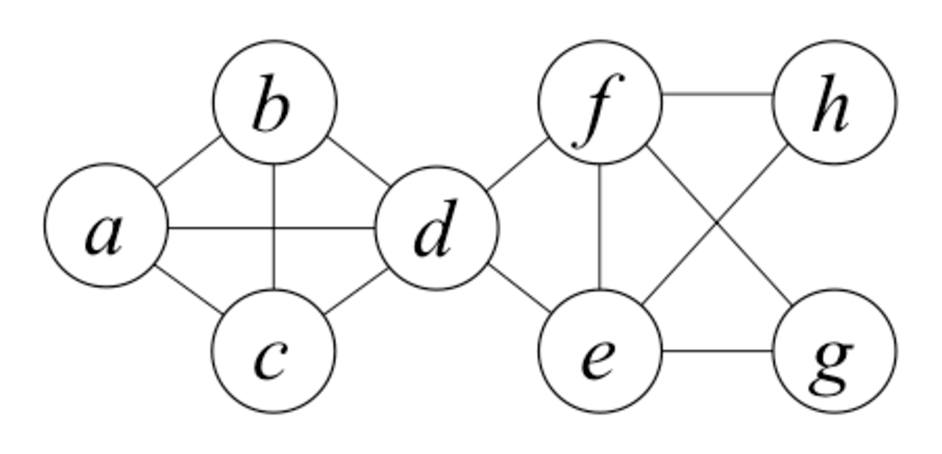
\includegraphics[scale=0.3]{./mcinfo_1.eps}
\caption{Graph of enumeration of maximal clique. 
Contains 4 maximal cliques \{a,b,c,d\}(id=0)、\{d,e,f\}(id=1)、\{e,f,g\}(id=2)、\{e,f,h\}(id=3).\label{fig:mcinfo_1}}
\end{center}
\end{minipage}

\begin{minipage}{0.5\hsize}
\begin{center}
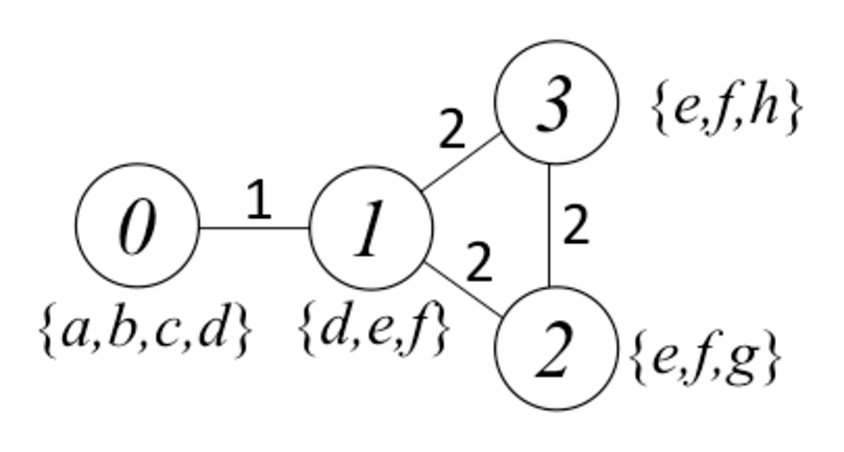
\includegraphics[scale=0.3]{./mcinfo_2.eps}
\caption{Maximal clique graph. The graph in Figure \ref{fig:mcinfo_1} shows clique id at the node. Edges with common nodes.
Clique id=1 is directly connected to 3 other cliques. Refer to section \ref{sect:mclique2g} if you want to output to graph format. 

\label{fig:mcinfo_2}}
\end{center}
\end{minipage}

\end{tabular} 
\end{center}
\end{figure} 

\begin{figure}[htbp]
\begin{center}
\begin{tabular}{c}

\begin{minipage}{0.5\hsize}
\begin{center}
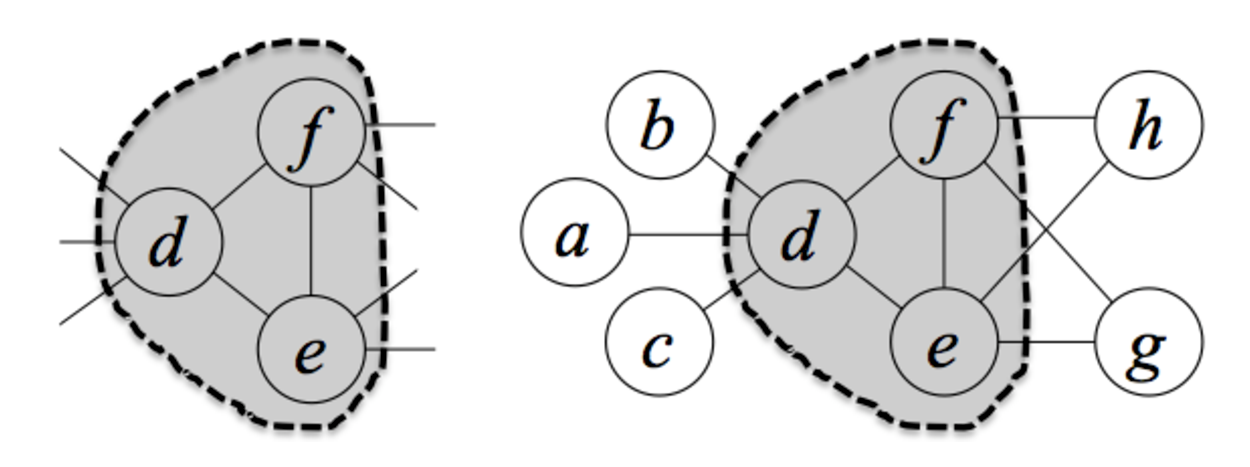
\includegraphics[scale=0.3]{./mcinfo_3.eps}
\caption{7 branches connects from clique id=1 (region shown in grey) to other nodes outside (left figure). 
Clique id=1 (region shown in grey) are connected to 5 nodes (right figure).
\label{fig:mcinfo_3}}
\end{center}
\end{minipage}

\end{tabular} 
\end{center}
\end{figure} 

Input data of this command is the same as the one used in mclique2g.rb command in section \ref{sect: mclique2g}, Table \ref{tbl: clique2g_1} shows the CSV formatted data consisting of two columns as cliqueID and node respectively. 
The output results are shown in Table \ref{tbl: mcinfo_3}, and information of maximal clique is shown in Table \ref{tbl:mcinfo_1}. 


\begin{table}[htbp]
\begin{center}
\begin{tabular}{cc}

\begin{minipage}{0.3\hsize}
\begin{center}
\caption{Input Data\label{tbl:mcinfo_2}}
{\small
\begin{tabular}{cc}
\hline
id&node \\
\hline
0&a \\
0&b \\
0&c \\
0&d \\
1&d \\
1&e \\
1&f \\
2&e \\
2&f \\
2&g \\
3&e \\
3&f \\
3&h \\
\hline
\end{tabular} 
}
\end{center}
\end{minipage}

\begin{minipage}{0.7\hsize}
\begin{center}
\caption{Output Results\label{tbl:mcinfo_3}}
{\small
\begin{tabular}{cccccc}
\hline
id&nSize&eSize&extNodes&extEdges&extCliques \\
\hline
0&4&6&2&2&1 \\
1&3&3&5&7&3 \\
2&3&3&2&4&2 \\
3&3&3&2&4&2 \\
\hline
\end{tabular} 
}
\end{center}
\end{minipage}

\end{tabular} 
\end{center}
\end{table} 



%これらのクリークと図に示された元のグラフとの関係について本コマンドは表\ref{tbl:ci_result}に示されるような結果を出力する。
%idはクリークを識別するIDで(図\ref{fig:ci_graph}のキャプションに記載)、それぞれのクリークについて表\ref{tbl:ci_flds}に示される情報を出力する。


\subsection{Format}
\begin{verbatim}
mcliqueInfo.rb i= [id=] [f=] [m=] [F=] o= [T=] [--help]
  i=     : File name of clique data
id=    : Field name of clique ID (default:"id") 
  f=     : Field name of node in clique (default:"node") 
  T= : Working directory (default:/tmp)
  --help : Show help information
\end{verbatim}

\subsection{Example}
\subsubsection*{例1: 基本例}

前節で解説した例。


\begin{Verbatim}[baselinestretch=0.7,frame=single]
$ more clique.csv
id,node
0,a
0,b
0,c
0,d
1,d
1,e
1,f
2,e
2,f
2,g
3,e
3,f
3,h
$ mcliqueInfo.rb i=clique.csv o=result1.csv id=id f=node
#END# /usr/bin/mcliqueInfo.rb i=clique.csv o=result1.csv id=id f=node
$ more result1.csv
id,nSize,eSize,extNodes,extEdges,extCliques
0,4,6,2,2,1
1,3,3,5,7,3
2,3,3,2,4,2
3,3,3,2,4,2
\end{Verbatim}


